%%%%%%%%%%%%%%%%%%%%%%%%%%%%%%%%%%%%%%%%%%%%%%%
%
% Template for Bachelor degrees
% DISI - Dipartimento di Ingegneria e Scienza dell’Informazione
% DISI - Department of Information Engineering and Computer Science
%
% update 2020-08-30
%
% To generate pdf 
% pdflatex __filename__.tex
% bibtex __file_name__.aux
% pdflatex __file_name__.tex
% pdflatex __file_name__.tex
%
%%%%%%%%%%%%%%%%%%%%%%%%%%%%%%%%%%%%%%%%%%%%%%%

% 2 side format
\documentclass[epsfig,a4paper,11pt,titlepage,twoside,openany]{book}
\usepackage{epsfig}
\usepackage{plain}
\usepackage{setspace}
\usepackage{multicol}
\usepackage[paperheight=29.7cm,paperwidth=21cm,outer=1.5cm,inner=2.5cm,top=2cm,bottom=2cm]{geometry} % layout setting
\usepackage{titlesec} % custom setup title of chanpter
% \usepackage{newtxtext,newtxmath} % times new roman

%%%%%%%%%%%%%%
% support for accented letters
%
%\usepackage[latin1]{inputenc} % Windows;
\usepackage[utf8x]{inputenc} % Linux (unicode package is required);
%\usepackage[applemac]{inputenc} % Mac.


%%%%%%%%%
% support for pics
\usepackage{graphicx} %package to manage images
\graphicspath{ {./graphics/} }
\usepackage[rightcaption]{sidecap}
\usepackage{wrapfig}
\singlespacing

% italian language
%\usepackage[italian]{babel}

\begin{document}

  % no page number
  \pagenumbering{gobble} 
  \pagestyle{plain}

\thispagestyle{empty}

\begin{center}
  \begin{figure}[h!]
    \centerline{
\psfig{file=marchio_unitrento_colore_it_202002.eps,width=0.6\textwidth}}
  \end{figure}

  \vspace{2 cm} 

  \LARGE{Department of Information Engineering and Computer Science\\}

  \vspace{1 cm} 
  \Large{Bachelor's Degree in\\
    Computer Science
    % Computer Science
    % Computer, Communication and Electronic Engineering
    % Information and Communications Engineering
    % Information and Business Organization Engineering
    % Electornics and Telecommunications Engineerign
  }

  \vspace{2 cm} 
  \Large\textsc{Final Dissertation\\} 
  \vspace{1 cm} 
  \Huge\textsc{ANALYSIS OF COST-EFFECTIVE INFLUENCE MAXIMIZATION STRATEGIES ON TEMPORAL NETWORKS\\}
  \Large{\it{}}


  \vspace{2 cm} 
  \begin{tabular*}{\textwidth}{ c @{\extracolsep{\fill}} c @{\extracolsep{\fill}} c}
  \Large{Supervisor} & \Large{Co-Supervisor} & \Large{Student}\\
  \Large{Paolo Casari} & \Large{Quintino Francesco Lotito} & \Large{Giacomo Casagranda}\\
  \end{tabular*}

  \vspace{2 cm} 

  \Large{Academic year 2021/2022}
  
\end{center}



  \clearpage
 
%%%%%%%%%%%%%%%%%%%%%%%%%%%%%%%%%%%%%%%%%%%%%%%%%%%%%%%%%%%%%%%%%%%%%%%%%%
%%%%%%%%%%%%%%%%%%%%%%%%%%%%%%%%%%%%%%%%%%%%%%%%%%%%%%%%%%%%%%%%%%%%%%%%%%
%% Note
%%%%%%%%%%%%%%%%%%%%%%%%%%%%%%%%%%%%%%%%%%%%%%%%%%%%%%%%%%%%%%%%%%%%%%%%%%
%% Thanks/ Acknowledgements section is optional
%%%%%%%%%%%%%%%%%%%%%%%%%%%%%%%%%%%%%%%%%%%%%%%%%%%%%%%%%%%%%%%%%%%%%%%%%%
%%%%%%%%%%%%%%%%%%%%%%%%%%%%%%%%%%%%%%%%%%%%%%%%%%%%%%%%%%%%%%%%%%%%%%%%%%
  \thispagestyle{empty}

\begin{center}
  {\bf \Huge Acknowledgements}
\end{center}

\vspace{4cm}


\emph{
A dutiful and heartfelt thank you goes out to all the people directly and indirectly involved in this journey and which I was lucky to be flanked to during its entire three years and a half duration. Without each of them it would not have been possible to complete it and enjoy all the satisfaction that it brought.\\
Firstly I want to thank Professor Casari, supervisor, and Doctor Lotito, co-supervisor, for allowing the realization of this work through their availability to follow me, professionality and precision to guide me and for all the knowledge transmitted to me.\\
I also want to thank my colleagues from the Computer Science course for all the good moments shared inside and outside the University and for the mutual help. Special thanks go out to Nicola, fellow student of mine for the past eleven years, with whom it has always been a pleasure to work and on whom I could always count. \\
Heartfelt thank you to my girlfriend Alyssa for being the closest to me despite the distance, for all the support and for always encouraging me to prove myself and keep going. I owe her much of this achievement for always being my biggest source of motivation for a year and a half now.\\
Thanks to my family for encouraging me to continue studying and allowing all this through the economic and moral support, for growing me and for all the teachings that made me become the man I am today.\\
Last but not least, a big thank you to all my friends for being there since day one, for all the good memories shared and for lightening all the stressful and difficult moments I have been through during this journey.}


  \clearpage
  \pagestyle{plain} % no heading, footer with centered page number

  
  % page number with Arabic format
  \mainmatter

%%%%%%%%%%%%%%%%%%%%%%%%%%%%%%%%%%%%%%%%%%%%%%%%%%%%%%%%%%%%%%%%%%%%%%%%%%
%%%%%%%%%%%%%%%%%%%%%%%%%%%%%%%%%%%%%%%%%%%%%%%%%%%%%%%%%%%%%%%%%%%%%%%%%%
%% Note
%%%%%%%%%%%%%%%%%%%%%%%%%%%%%%%%%%%%%%%%%%%%%%%%%%%%%%%%%%%%%%%%%%%%%%%%%%
%% The maximum number of pages is 30, including:
%%   index
%%   abstract
%%   chapters
%% Excluding:
%%   frontispiece
%%   acknowledgements 
%%   attachments
%%
%% For further details and updated rules, please check the guidelines.
%%%%%%%%%%%%%%%%%%%%%%%%%%%%%%%%%%%%%%%%%%%%%%%%%%%%%%%%%%%%%%%%%%%%%%%%%%
%%%%%%%%%%%%%%%%%%%%%%%%%%%%%%%%%%%%%%%%%%%%%%%%%%%%%%%%%%%%%%%%%%%%%%%%%%

    % index
    \tableofcontents
    \clearpage
    
    
          
    % group to define space between chapters
    \begingroup
      % no page break between chapters
      % override clear page commands
      \renewcommand{\cleardoublepage}{} 
      \renewcommand{\clearpage}{} 
      % override format of title chapter
      % from
      %   Chapter X
      %   Title
      % to
      %   X   Title
      
      \titleformat{\chapter}
        {\normalfont\Huge\bfseries}{\thechapter}{1em}{}
        
      \titlespacing*{\chapter}{0pt}{0.59in}{0.02in}
      \titlespacing*{\section}{0pt}{0.20in}{0.02in}
      \titlespacing*{\subsection}{0pt}{0.10in}{0.02in}
      
      % summary / abstract
      \chapter*{Abstract} % no number
\label{abtract}

\addcontentsline{toc}{chapter}{Abstract} % add to index
Complex networks are amongst the most studied branches in computer science, not only because of the vastity of the topic itself, but also because of their strong connection with other disciplines such as economics, biology, politic sciences and many others. Modern-day social networks enhance these correlations even more, thanks to the fact that they are stable in every human's daily life whether it's related to work, news or simple leisure activities. This work is focused on social networks Influence Maximization (IM), a widespread algorithmic problem that has been studied frequently as social networks have been expanding for years, where the goal is to find the optimal seed set K of a network that can maximize the spread of an influence. This has been studied under several points of view in the recent years since it has a big range of practical applications not only in computer science (i.e., fake news epidemics), but also in Economics (Viral Marketing), Sociology and more. 
Social networks are modeled through mathematic graphs, an easy and functional structure where nodes represent the users and edges represent the interactions happening between two users, for example a message.
\\
\\
However a limitation of classical Influence Maximization Frameworks is that they are often based on some assumptions, like modeling social networks through static graphs. Obviously, every spreading process occurs over time, and as the time progresses social networks do evolve quite drastically as shown in studies by Marlyne Meijerink-Bosman et. al. Temporal Graphs are introduced, to easily assign each edge a timestamp to model a realistic dynamic social network interaction. A temporal graph can be interpreted as a set of static graphs that model the evolution of the network over time, with nodes joining, leaving and interacting with each other. Another limitation of many IM works is the general purpose of limiting the seed set size, but not restricting the effective choice of the single nodes; it is not realistic to model an influence maximization framework assuming that nodes have equal seeding cost. Just by considering viral instagram marketing, a more influential user requires more money to make an endorsment of a product, compared to people with less network presence. A function that models the node cost dynamically is required. On top of that, optimization algorithms proposed in existing IM studies have very large computational costs, which makes them not suitable to big scale networks, like today's social networks are.
\\
\\
This work aims at presenting a new, more realistic influence maximization framework since generally proposed solutions for IM are optimal but can’t really be applied in realistic scenarios since there are many factors to take into consideration, such as restricted freedom on the seed set choice. A suitable model that takes into account all of the above is proposed and different seeding strategies are built after extracting the most relevant features from different temporal network models. The results are obtained by testing each strategy on different realistic networks and then discussed and contextualized.

The work done is summarized by these points below:
\begin{itemize}
\item Research of the existing studies regarding the subject
\item Analyzing the problem from a more realistic perspective with the appropriate constraints
\item Coding python scripts to create the base structure, the simulator and the solution algorithms
\item Analyzing different solution ideas for the different network models 
\item Testing those solutions on realistic networks and comparing the performances
\end{itemize}








      \newpage
%%%%%%%%%%%%%%%%%%%%%%%%%%%%%%%%%%%%%%%%%%%%%%%%%%%%%%%%%%%%%%%%%%%%%%%%%%
%%%%%%%%%%%%%%%%%%%%%%%%%%%%%%%%%%%%%%%%%%%%%%%%%%%%%%%%%%%%%%%%%%%%%%%%%%
%% Note
%%%%%%%%%%%%%%%%%%%%%%%%%%%%%%%%%%%%%%%%%%%%%%%%%%%%%%%%%%%%%%%%%%%%%%%%%%
%% The abstract is a short summary of the work describing the target,
%% the subject of the thesis, the methodology and the techniques,
%% the data collection and elaboration, the explanation of the
%% reached results and the conclusion.
%% The abstract of the dissertation must have a maximum length of 3 pages
%% and must include the following information:
%%   context and motivation
%%   short summary of the main problem you have dealt with
%%   developed and /or used techniques 
%%   reached results, the personal contribution of the student has to be highlighted
%%%%%%%%%%%%%%%%%%%%%%%%%%%%%%%%%%%%%%%%%%%%%%%%%%%%%%%%%%%%%%%%%%%%%%%%%%
%%%%%%%%%%%%%%%%%%%%%%%%%%%%%%%%%%%%%%%%%%%%%%%%%%%%%%%%%%%%%%%%%%%%%%%%%%      
      
      %%%%%%%%%%%%%%%%%%%%%%%%%%%%%%%%
      % chapters
      %
      % \input or \include
      %
      \chapter{Complex Networks}
\label{cha:intro}

Networks constitute the backbone of any complex system
\cite{10.5555/3181286}, from the human brain to transport infrastructures, online social systems and financial markets. Characterising their structure and behaviour improves our understanding of the phenomena that shape the world we live in and its society. Complex networks are systems consisting of a high number of units (nodes) interconnected through highly non-trivial interaction patterns. The human brain, social systems, both on and off the Internet, are common examples of complex systems modelled through complex networks but other examples like water distribution, transport systems and blood flux show that complex networks are all around us and shape nearly everything we are surrounded with nowadays, from metabolic to online systems. One of the key features of complex networks is that they often exhibit a degree of clustering, meaning that nodes tend to be highly connected to other nodes that are nearby in the network. This can lead to the formation of small, tight communities within the larger network, i.e. social communities and friendship groups. Another important feature emerged from studies of complex networks \cite{articl2e} is that they often exhibit a power-law distribution of node degrees, meaning that there are relatively few highly connected nodes (hubs), and many more nodes with relatively few connections. On social networks, this is the case of influencers. This makes understanding complex networks extremely important and so are all the developments in this branch, whose results have been already proven to have a huge impact on practical disciplines.

\begin{center}
    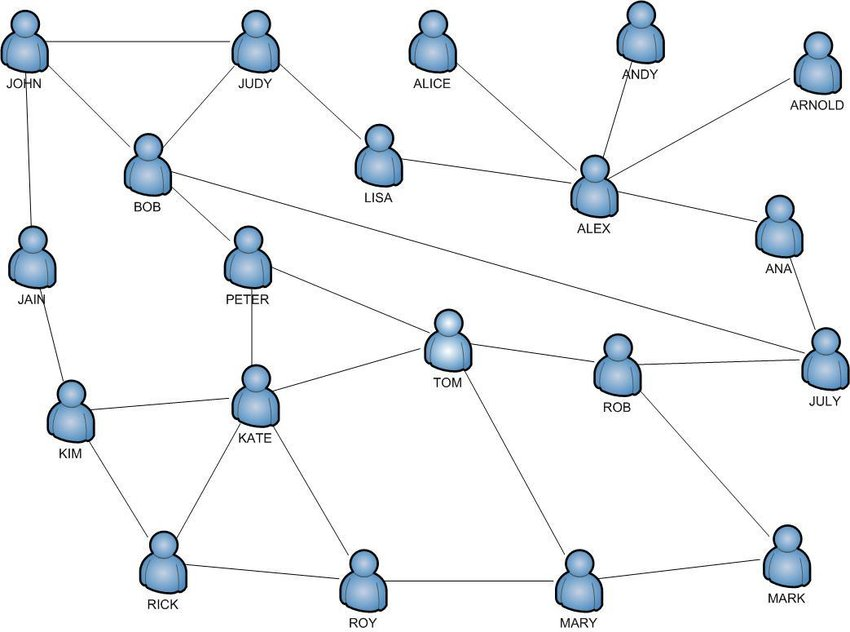
\includegraphics[scale=0.4]{complexnet}
    \\
        Figure 1.1: Social Interation Complex Network
\end{center}

\section{Graphs}
\label{sec:graphs}
The mathematical interpretation of networks is given through what's called graph theory. A network can be seen as a Graph(N, E) composed of two sets: N is the Node Set, consisting of all the users/hosts of the network, and E is the Edge Set, consisting of all the interactions that happen between two users, whether it's talking, messaging, physical or abstract connection. Given an interaction between nodes A ad B, it is going to be represented by the Edge (A, B). Nodes connected by an edge are said to be adjacent (or neighbors), and a node's degree is defined as the number of edges incident to that node. The concept of degree is really important to identify previously described hubs in a network and understand how information can flow throughout a network. A graph can be directed if the interactions are shaped so that it is possible to identify a source and a destination, i.e., a message graph, or undirected, i.e., a friendship graph where the interactions are mutual. When working with directed graphs it is essential to highlight the difference between in-degree (how many edges go into a node) and out-degree (how many edges go out from a node).

\begin{center}
    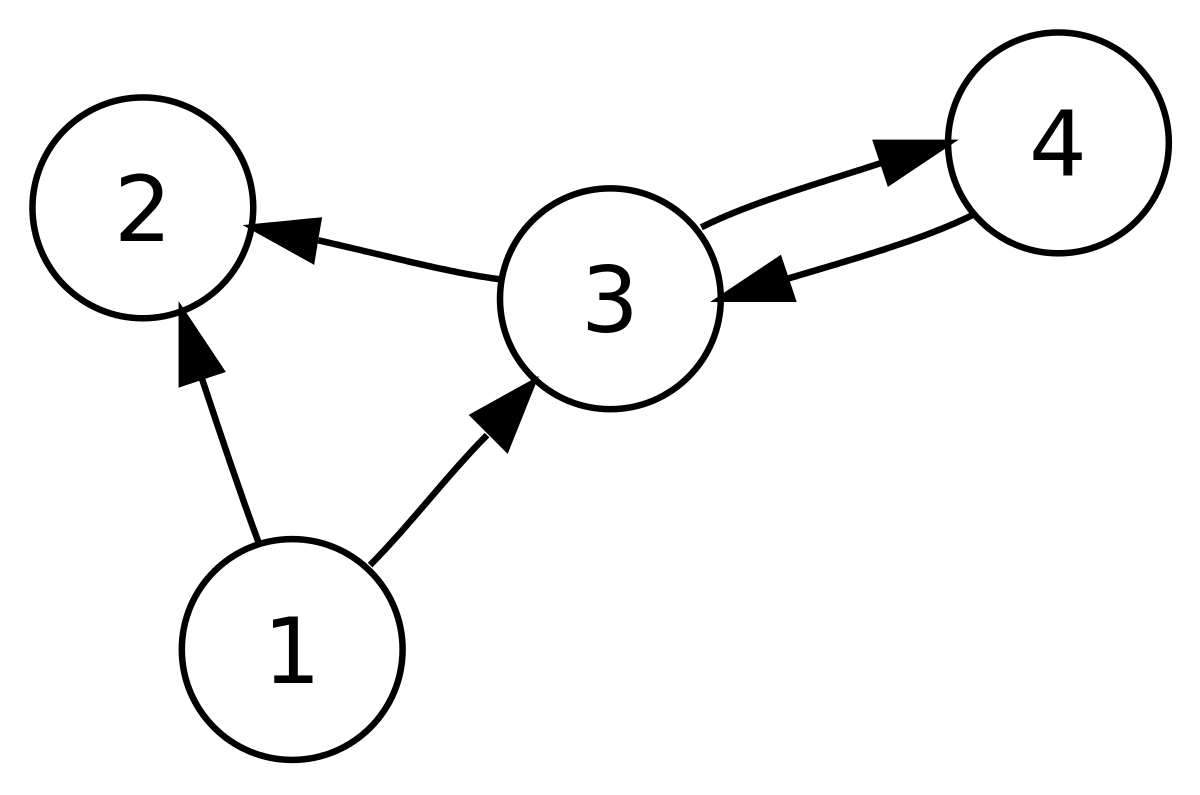
\includegraphics[scale=0.1]{graph}
    \\
        Figure 1.2: Directed Graph Overview
\end{center}

\section{Temporal Networks}
Temporal networks or dynamic networks are complex systems that change over time. Studying temporal networks fills the gap between network science and time-series analysis area\cite{HOLME201297}. 
This necessity of introducing the temporal aspect comes from the fact that nearly everything in the world is time-related, especially complex networks. From social networks to biological phenomena mostly, everything that is considered a complex system is subject to somewhat evolution over time\cite{PMID:35538294}. 
Social interactions are the clearest example, as new friendships might be introduced or cancelled, and the possibility of social interactions through the Internet has eased that by a lot.

\subsection{Dynamic Edge Set}
\label{sec:dygraphs}
As mentioned before a network can be thought of as a graph. In Dynamic networks, the Edge set can vary over time meaning every single interaction happens at a time T, which comes in as an Extra parameter for the edges. This means that Edges are identified now by a 3-tuple (source, destination, time). To give a better representation of a dynamic network edges can be grouped by discrete time so that every interaction in a time group W happens at that specific time, or inside that specific time window. After that groups are sorted by time and for each of them a static graph is created, with every Node of the network but only the Edges belonging to that group. Confronting each of those static graphs in order of time evolution gives an easy ad precise overview of the changes that the network has been through during the course of time.

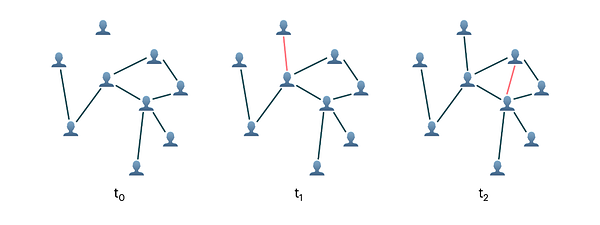
\includegraphics[scale=0.8]{temporalnetwork}

\begin{center}
    Figure 1.3: Temporal Network Change Overview
\end{center}

Isolated Nodes can be seen as “offline” users, while connected Nodes can be seen as “online” users interacting with some other online user(s) at that specific time. 

\subsection{Graph Concepts Adaptation}
\label{sec:dygraphs2}
The study of temporal networks is extremely important to have a better representation of the real-world systems that change throughout time. However, new challenges are brought up by the fact that introducing temporal networks adds one dimension to the data, making it not only harder to manage but also completely impacting even the basic notions of graphs. Every concept needs to be adapted when dealing with temporal networks. New algorithm design is then needed, with some problems being natural extensions of static graph problems to a temporal perspective and others being new problems being risen by the temporal evolution aspect. 
Not only the basic system structure but also the common concepts like node degree and adjacency now assume different values based on the discrete-time we are considering. On static unweighted graphs, a node degree is defined as the number of edges incident to that node and indicates both the total number of interactions and the number of nodes the node interacts with. Temporal networks allow for multiple Edges between the same pair of Nodes, similar to multi-graphs and weighted graphs, marking a clear distinction between the number of total interactions and the number of users interacted with. Reachability and path finding are now crucially related to the edges' effective presence at a discrete time and most importantly to their overall ordering, as shown in studies by Huanhuan Wu et. al about fath finding in temporal graphs.
\cite{10.14778/2732939.2732945}

\section{Social networks}
\label{sec:socialnetworks}
Social networks are large scale online networks that have become extremely powerful tools thanks to their ability to connect people and link disconnected networks together. They also allow for easier, effective and multiple interactions between people. This makes data flow very well through a social network thanks to the propagation that comes with interaction between the users in the form of ”word-of-mouth” communications. Information can flow in different ways through a social network, either through conversations between users and also through each user's feed, that depends on the user's following/friendship users set. Notice how simple directed temporal graphs can be used to model a social conversation network, whilst for interactions between multiple users it is needed to introduce higher order structures such as hypergraphs, that can better represent social networks adding group dynamics. However that increases the complexity of the data, so this work is limited to dual users conversations network, that can still provide a good amount of information spread, expecially through fast spreading informations like rumors\cite{10.2307/45018860}.


      \newpage
      \chapter{Epidemics and Influence Maximization in Complex Networks}
\label{cha:2}
Influence Maximization is an algorithmic problem in complex networks \cite{SINGH20227570}. The problem consists of finding the best Seed Set K of a Network so that the spread of influence is maximized at the end. We are interested in maximizing the number of total influenced nodes.
This makes social influence problems very important since their range of application is enormous, going from viral marketing to disease and fake news epidemic spread. A good example of practical application in Viral Marketing is choosing the best influential users on the social network to endorse a product, to maximize the interest in that product across the whole network. What follows is an analysis of the related works on influence maximization that inspired this thesis. \\
Studies on clusters like \cite{articl2e} are extremely useful for the characterization of the network and feature extraction, useful for developing solutions for specific algorithmic problems. The work that mostly inspired this thesis is the study by Sirag Erkol et. al \cite{unknown} that extends the common greedy algorithm for static network influence maximization to a temporal perspective. This work is based on a similar infection model, but oriented towards a more realistic and less optimal direction that can better fit a realistic situation.
\\
 
\section{SI Model}
\label{sec:si}
The network is modeled through a Susceptible-Infected model
\cite{MORE2019102}. That is the simplest form when talking about disease models, since it does not include recover dynamics, but for the sake of IM those are just random probabilities that limit the overall performance, but do not play any key role when selecting the best initial Seed Set. It also allows spreading on single interactions, unlike models where the influence only affects a node based on how much the same influence is spread among his neighbors.
In a SI model every node is either in a Susceptible (neutral) or Infected state, and cannot revert once it enters the second one. Every node is Susceptible at time zero, except the Seed Set nodes that are set to Infected. Every time an Infected node interacts with a Susceptible one according to the network there is a fixed probability Pspread of that second node becoming Infected as well. On the current implementation an eventual failure of spreading between two nodes does not affect the second node's probability of being infected in the future (fixed probability).
Future works aim at extending the simulation context by adding recover dynamics and also dynamic probability and trust dynamics between nodes.

\begin{center}
    
\includegraphics[scale=1]{simodel}
\end{center}


\begin{center}
    Figure 2.1: Susceptible-Infected Model
\end{center}

\section{Related Work and Optimal Solutions}
\label{sec:litreview}
Influence maximization has been widely studied since it's extremely important to identify the most influential seed set in a complex network. Optimization solutions have been proven to be NP Hard, the goal of this work is to measure and compare the performance of quicker and possibly sub-optimal solutions under more realistic circumstances not considered in existing works. 

\subsection{SI Influence Maximization On Static Networks}
\label{sec:static}

Most of the existing work on influence maximization is based on the assumption of the network being static. The optimization algorithm is greedy \cite{article}, and gradually builds the Seed Set by adding the node that can better improve the influence spread of the current Seed Set; this can be either calculated or estimated each time, meaning that the algorithm will be NP-Hard. Quicker algorithms that can give good performance can be built on the same greedy base but using easier graph concepts to estimate a node’s influence, for example degree centrality. 
The work proposed deals instead with dynamic (or temporal) networks, that can represent a social network in a better way considering the fact that not every user is connected at the same time.

\subsection{SI Influence Maximization On Temporal Networks}
\label{sec:dynamic}
Many studies of Influence maximization are limited to static networks that do not change through the time; this can be restrictive because often interactions change over time in a highly dynamic manner. The optimization solution in temporal networks is a natural extension of the greedy algorithm for static networks\cite{unknown}, however when working with non-optimal solutions, like this work does, it is not possible to predict exactly how much a node is going to contribute to influence. That is because influence starts from a Seed Set but is then propagated through a cascade based on the interaction between the nodes. Furthermore, in temporal networks the cascade follows some time order, meaning that there are nodes that activate earlier than others, so in those scenarios it is not only important to consider the “popularity” of a node, but also how it can impact the whole cascade. Notice that, in order to analyze that aspect, full knowledge about the network (nodes, size) and its evolution is needed, otherwise it is essential to implement algorithms to predict the network changes. In a study by H. Zhuang et. al \cite{inproceedings} are proposed some algorithms to probe the network at a time t with no knowledge and predict the full network structure at that time by reconstructing it through the probing data and the information about the previous stages. However, this dissertation is based on having full network knowledge, and will take into account all the just discussed variables, that depend on the network structure, combining them with realistic general influence variables such as a limited budget, cost of selecting an initial node, and spreading probability.

\subsection{Seed Set and Cost}
\label{sec:dycost}
Most of the existing works on influence maximization aim at finding a generally small number of initial nodes, by setting a maximum cardinality k to the initial Seed Set and building it gradually through greedy approaches. This makes seed sets to be all made of k nodes, with chosen nodes being characterized by the different solution algorithms.  When trying to expand seeding to a more realistic scenario, it is inevitable to give each node a different cost depending on his role inside the network. Viral Marketing is a clear example of that, where we obviously need more budget to make some product be advertised by some famous influencer(s).
This works proposes dynamic costs for each node, depending on his degree in the network, and a fixed budget cap is introduced. This allows the seeding to be more realistic and various in both size and nodes selected. The idea here is that the more a network node is influent (interacts with other nodes) the more his cost to be initially selected grows. This is why the exponential function is used to dynamically compute the cost of a node, this way nodes with higher degree are always going to be out of budget, encouraging the usage of more marginal nodes to see how well they can do based on the network structure.
The cost of a node n is calculated as follows:
\begin{center}
    $c(n) = {\rm e}^{\delta(n)} \, ,$
where $c(n)$ is the cost of node $n$, and $\delta(n)$ is its degree
\end{center}
Note that this also never allows a node's cost to be zero.
\\
Depending on the structure of the network (number of nodes, edges) different simulations with growing budgets are performed for each strategy to measure how good it works. The goal of this work is to study how far we can spread our influence on different networks with extremely limited budget.

\subsection{Network Knowledge}
\label{sec:input}
This dissertation, along with almost all the existing works on influence maximization, works on the assumption that full network knowledge is given, as well as full information on when and how it evolves through the time. 

\section{Proposed Work}
\label{sec:proposed}
The dissertation will bring an unique realistic aspect when developing a seeding strategy on a complex temporal network. It will cover the temporal aspect of the network, as well as a constraint on the maximum budget available to select the nodes to be infected at the beginning. The  network is modeled with a Directed Graph, and a classic SI model is used for influence maximization, hence the influence happens through the interaction between different nodes in the network, starting from the selected K initial nodes. Furthermore, this work aims at proposing and measuring the performance of non-optimal strategies that can be applied to large-scale realistic networks under severe budget restrictions.








      \newpage
      \chapter{Technologies and Implementation}
\label{cha:tech}
The chapter covers the whole structure of the Python script used to both create the support model and also the simulator to measure the performance of each infecting strategy.

\section{Python}
\label{sec:python}
Everything is implemented through  a Python Program that allows to fetch the data, create the core structure of the network, compute functions, implement the seeding strategies and obviously run the simulations to measure the results and plot them to give graphic user friendly representations of the results.
A few support libraries are used for the above mentioned implementations, including:
\begin{itemize}
\item DyNetX to create the core network structure
\item MatplotLib to display a single simulation's result through a line chart (number of Infected nodes over time)
\item Math and Random to compute functions and generate random probability values
\end{itemize}

\subsection{DyNetx Library}
\label{sec:dynetx}
The Network is designed as a Temporal Directed Graph G. To do that DyNetX is used. It is a free open source Python Library that implements data structures to create and analyze temporal networks. The library is based on Networkx, and adds the temporal feature to all the data structures. This makes it extremely user friendly since it extends all common graphs concepts and methods to bring them to a temporal context. Some useful DyNetX methods include:
\begin{itemize}
\item Automatically build a dynamic graph from a text file
\item Compute Node Degree at a specific time or time window
\item Slice a Graph in time windows, or extract sub graphs at specific time or time window
\end{itemize}

\subsection{Network Nodes}
\label{sec:nodes}
Nodes are represented as Objects, with respective Id, Status and Cost as main attributes. Other attributes such as degree and neighbors are not needed as they can be easily computed dynamically and are not of common interest in all the proposed solutions, and are therefore computed and/or stored in memory only when needed. Id is fetched from the dataset while status and cost are initialized to Susceptible and zero. Status is then set to Infected for the selected Seed nodes, while cost is calculated for each node through the next mentioned loop.

\section{Script Structure}
\label{sec:script}
The script is coded to sequentially perform the following actions:
\begin{itemize}
\item Parse a dataset and build a Dynamic Directed Graph
\item Loop through each node to compute its cost to be selected in the initial Seed Set
\item Select a proposed strategy (selecting Pspread and total budget values)
\item Change the state of the Seed nodes to Infected
\item Run the simulation and display the run's result with an easy line chart to show the Influence Progression over time

\end{itemize} 
\hrule 
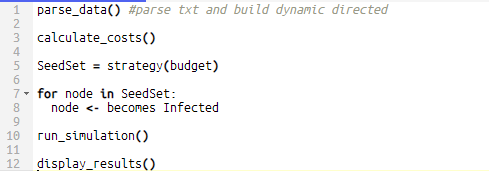
\includegraphics[]{script_structure}
\hrule

\begin{center}
    Figure 3.1: Pseudo code sum up for the entire script
\end{center}

\subsection{Simulation and Results Display}
\label{sec:run}
The simulation algorithm is implemented following the time order of the Network itself. Given the Seed Nodes as Infected and all the other ones as Susceptible, nodes interactions are scanned in ascending order. Whenever an interaction is recognized to be happening from an Infected node to a Susceptible one, the Susceptible node changes its state to Infected with fixed probability Pspread. At any time change information about the Influence progress is fed to the plot so that the final display can also better cover the Influence curve, to show the Infection progress very clearly throughout the time.
\\
\hrule 
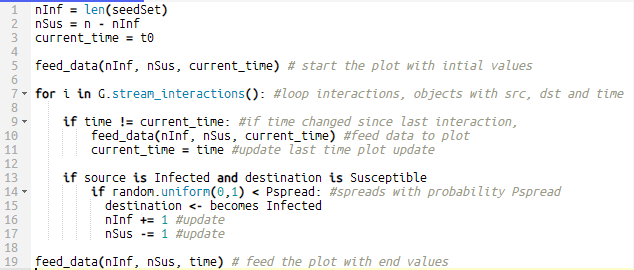
\includegraphics[]{code_simul}
\hrule

\begin{center}
    Figure 3.2: Pseudo Code for Simulation Run
\end{center}

The Single Simulation Plot allows the user to really see in detail how the curve of the Infection evolves throughout the time. This is interesting not only for the fact that it gives a visual representation of the result but also because it can underline the difference between different strategies and different network types. \\

\begin{center}
    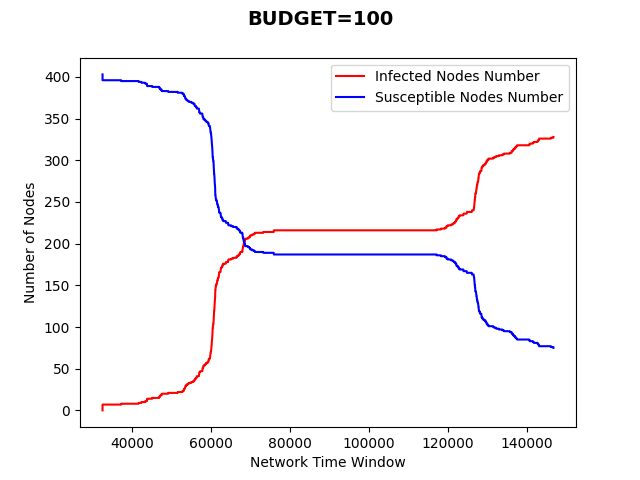
\includegraphics[scale=0.8]{line chart}\\
    Figure 3.3: Final Display of The Single Simulation Results
\end{center}

When working with temporal networks each interaction happens at a discrete time and so is everything that comes with it like nodes changing their state and network state update; this means that network structure and seed selection play a crucial role in determining the type of curve of infection. It can space anywhere between being a slow progressing curve or an early spiked curve. This allows strategies that aim at creating an early spike curve to maximize the time window where Infected users are actively interacting with the network, rather than "wasting" potential time and all the interactions that might occur in that window.\\



      \newpage
      \chapter{Network Types and Solutions Proposed}
\label{cha:netsolutions}
As mentioned earlier in this dissertation, optimal solutions have high computational cost whilst the algorithms proposed in this work can be applied to large scale networks; when working with these kind of solutions it is not possible to exactly know which node is going to contribute best to the influence spread. However, full network knowledge is still given and it is possible to use it to extract the basic features that characterize that network, and therefore estimate the expected diffusion value of a node based on its properties and role in the network. The proposed solutions consider the following aspects when deciding the best nodes to choose:
\begin{itemize}
\item Node Activity, based on the node's degree
\item Node Spread Paths, based on how wide is the reach of the cascade originated by every node
\item Node Activation, based on node reachability
\item Node Temporal Position, based on how much of the time window the node affects
\end{itemize}

Different strategies are proposed, some considering more activity based characteristic like node degree and some focusing more on the temporal aspects of the network, like node coverage and activation time. The goal is too measure the performance of those strategies on different networks, each of them varying in size, and edges' frequency and temporal distribution. After analyzing the results it is possible to see if non optimal solutions proposed under these realistic network and budget conditions can still produce a good influence spread, and compare which strategy works best under some specific network circumstance.

\section{Network Datasets}
\label{sec:data}
The strategies are evaluated on realistic temporal network Datasets all based on interactions between two people, presented here:
\begin{itemize}
\item Message Dataset (College) - 1899 nodes, 59835 edges, start time 1082040961, end time 1098777142, no simultaneous edges
\item Proximity Conversation Dataset (Ia) - 113 nodes, 20818 edges, start time 20, end time 212360, presence of simultaneous edges
\item Chat Dataset (SFHH) - 403 nodes, 70261 edges, start time 32520, end time 146820, presence of simultaneous edges
\end{itemize}

\section{Network Features}
\label{sec:necfeats}
Networks are always different from each other, because of the size and the number and concentration of the edges/users. However studies about small world properties \cite{https://doi.org/10.48550/arxiv.2103.08035} prove that seemingly random networks have some type of correlation. These facts are even more emphasized in temporal networks, because they can be interpreted as a sequence of static networks. This means that not only the size and the concentration of the network can vary but also the distribution of the edges over its time window. Networks can be roughly grouped following those key aspects:
\begin{itemize}
\item Highly/Lowly Connected Networks
\item Homogeneous/Heterogeneous Networks
\item Unreachable/Isolated Nodes Networks
\item Time Balanced/Unbalanced Networks
\end{itemize}

\subsection{Highly Connected Networks}
\label{sec:hynets}
These kind of Networks are characterized by a higher edges to nodes ratio; this means that the average number of outgoing edges per node in the network is higher. Notice how in our specific study scenario, with limited budget, this can not ensure us any preliminary expectation about any influence spread because we don't know how the average degree of the nodes is actually distributed, and with limited budget we could be able to select only the nodes with way below average degree.  
The Proximity Dataset and the Chat Dataset are good examples of that since they have an high edges to nodes ratio of well over 100: however they do differentiate in terms of the number of nodes, meaning that in the Ia Dataset there are more interactions that occur multiple times at different timestamps. 
\begin{center}
    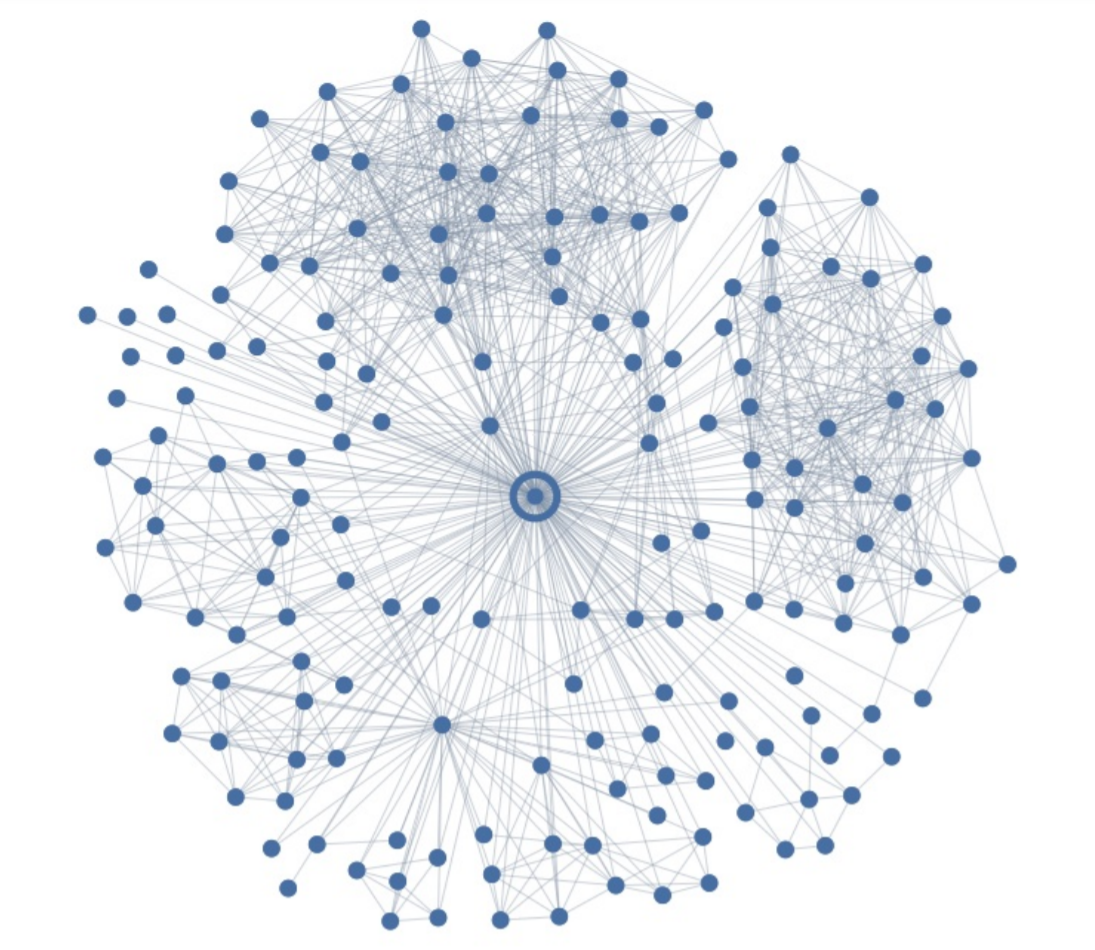
\includegraphics[scale=0.2]{highconets}
    \\
    Figure 4.1: Highly Connected Network Overview
\end{center}

\subsection{Lowly Connected Networks}
\label{sec:lownets}
These kind of Networks are characterized by a lower edges to nodes ratio: this means that the average number of outgoing edges per network node is lower. Generally we expect the worst influence spread in these kind of networks, because if there are few nodes with higher degree they are probabily going to be unaffordable, and on the other hand if the edges are distributed in a uniform way among the nodes, they are going to be very low in number.
\begin{center}
    
\includegraphics[scale=0.8]{lowconets}
    \\
    Figure 4.2: Lowly Connected Network Overview
\end{center}

\subsection{Unreachable/Isolated Nodes Networks}
\label{sec:isonets}
A node is said to be isolated when it has no edges pointing in and out of himself, hence both its in degree and out degree are zero. An unreachable node is a node whose in degree is still zero, however he has some edges pointing out of him and therefore can be useful to spread influence. This can be also common in lowly connected networks. In some networks with a higher number of unreachable nodes it might be worth to consider infecting some of them, other wise they are going to be cut out of the network forever.

\begin{center}
    
\includegraphics[scale=0.5]{isolated}
    \\
    Figure 4.3: Isolated/Unreachable Nodes Network Overview
\end{center}


\subsection{Time Balanced/Unbalanced Networks}
\label{sec:timenets}
Temporal Networks hide some problems related to node reachability: some nodes might be accessible only at certain times, and according to the network's temporal structure these times can be located earlier in the time window or later. The earlier those times are, the more difficult it is to reach a node, because there is less time for other interactions to happen that can generate a cascade leading to that node, whilst if a node can directly be accessed only at a later time step, there is more probability of other nodes activating earlier who can generate a cascade that includes that node. This obviously depends entirely on the network structure and the users interactions.
On top of that, time plays a key factor in the growth of the spreading curve. Different strategies that infect different nodes are going to develop differently, and given full network structure it is possible to make some observations and differentiate between nodes who can contribute a lot, and nodes that can contribute earlier and use as much time as possible. This is also enhanced by the fact that time is not related to the node cost in our modeled system, while degree is.

\begin{center}
    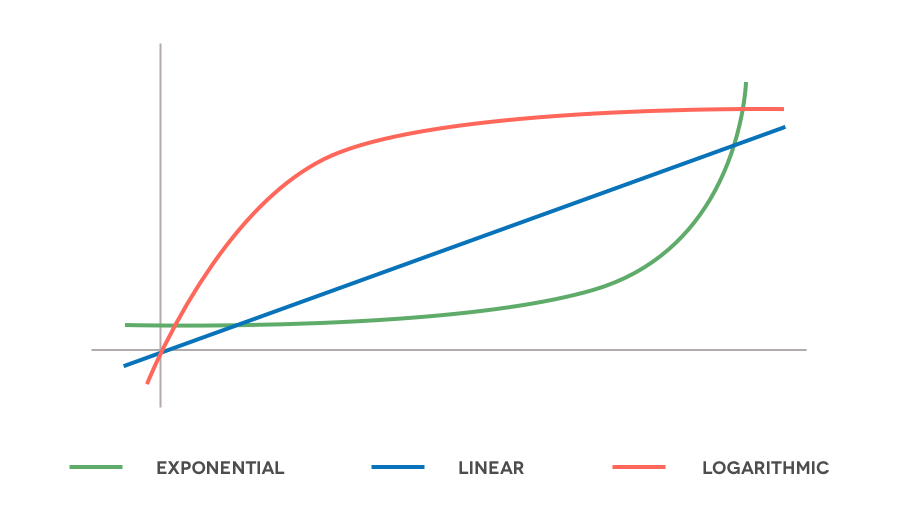
\includegraphics[scale=0.5]{curves}
    \\
    Figure 4.4: Different curves with different growth speed
\end{center}

\section{Influence Maximization Strategies}
\label{sec:strats}
In this section, we introduce the strategies implemented and studied. Each strategy is based on some possible network feature, with some of them being natural extension of static influence maximization strategies and some other strongly based on the temporal aspect of the network.
Each strategy was slightly optimized by not allowing to select two nodes with common neighbors. This enables an optimal usage of the budget along with good initial node coverage. What follows is a list of the strategies with a brief explaining of the idea behind the strategy, its code and how its characterized.

\subsection{Highest Degree Nodes (HDN)}
\label{sec:stratgreedy}
The idea behind this strategy is the simplest among all: we try to estimate the expected diffusion value of a node through its activity in the network, the more it interacts the more it can spread influence. It's greedy oriented and it is implemented to have a final clear report of how important it is to consider the time factor to estimate a node's expected diffusion value. Although this strategy might look pretty solid on the most basic influence maximization frameworks, there are some drawbacks:
\begin{itemize}
    \item Nodes with higher degree have higher cost, which means this strategy tends to build rather small seed sets
    \item Cost is not optimized. Given the exponential function to compute a node cost, picking a node with degree k costs more than picking two nodes each of them with degree k/2
    \item Temporal aspect is absolutely ignored. If the selected nodes interact only at the last time steps of the network almost every edge is wasted, resulting in poor performance
\end{itemize}

\begin{center}
    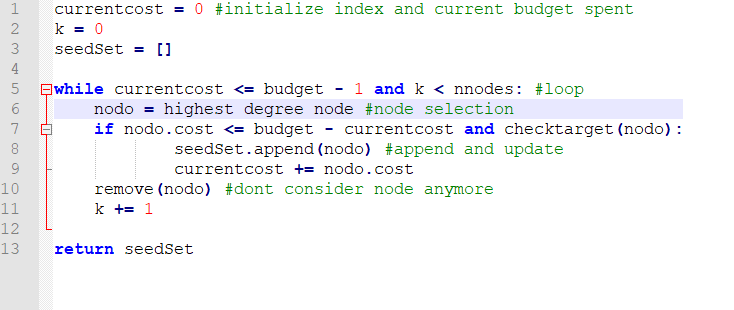
\includegraphics[scale=0.6]{/PseudoCode/greedy}
    \\
    Figure 4.5: Pseudo code For HDN function
\end{center}

\subsection{Highest Degree's Cheapest Neighbor (HDCN)}
\label{sec:stratneighbors}
This strategy is born after the main drawbacks of the First One. Here, the idea is to mitigate the cost, by trying to affect one of the neighbors of the highest degree node in order to try and save budget. This strategy ignores temporal aspects as well, as it just aims at seeding the cheapest among the neighbors, to secure more seed nodes given the fact that cheap nodes are more budget effective. 

\begin{center}
    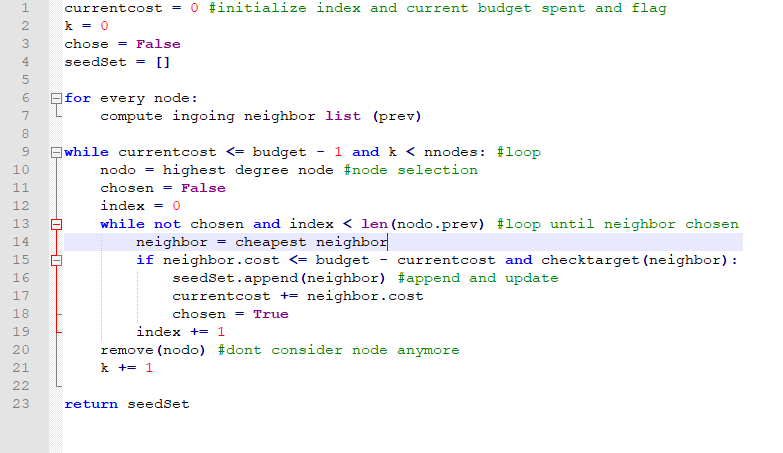
\includegraphics[scale=0.6]{/PseudoCode/neighbor}
    \\
    Figure 4.6: Pseudo code For HDCN function
\end{center}

\subsection{Earlier Nodes (EN)}
\label{sec:strattimeorder}
This strategy is purely based on the temporal aspect of the network. It also follows a greedy approach but adds the nodes that appear earlier in the network interactions, to maximize the influence and the time span used. The strategy does not take into account node degree at all (unless earlier nodes are tied in time), so the degree of the first nodes impact the strategy's overall performance.

\begin{center}
    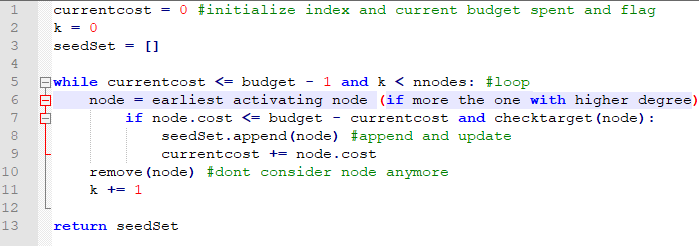
\includegraphics[scale=0.9]{/PseudoCode/early}
    \\
    Figure 4.7: Pseudo code For EN function
\end{center}

\subsection{Unreachable, Time Oriented Nodes (UTON)}
\label{sec:strattimeiso}
The idea behind this strategy is to take advantage of highly connected networks, where reachable nodes are well connected each other. The strategy aims at seeding the nodes that have less probability of being reached, with unreachable nodes (if any) being the first nodes to be seeded. When more unreachable nodes, the earliest to activate are taken first. This strategy allows to include nodes that would get easily cut out of the network, but does not consider node degree.

\begin{center}
    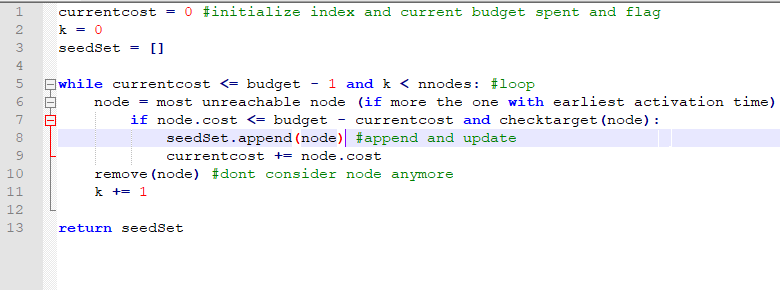
\includegraphics[scale=0.8]{/PseudoCode/unreachtime}
    \\
    Figure 4.8: Pseudo code For UTON function
\end{center}

\subsection{Unreachable, Degree Oriented Nodes (UDON)}
\label{sec:stratdegreeiso}
This strategy is a variant of the previous one, but here multiple unreachable nodes are taken first the higher their degree is.  This strategy allows to include nodes that would get easily cut out of the network, but relies more on a degree factor rather than a temporal one.

\begin{center}
    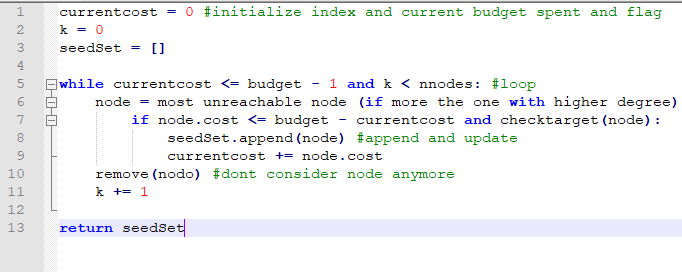
\includegraphics[scale=0.9]{/PseudoCode/unreachdeg}
    \\
    Figure 4.9: Pseudo code For UDON function
\end{center}

\subsection{Max Cover Nodes (MC)}
\label{sec:maxcover}
The final proposed strategy, as its name says, aims at maximizing the ideal cover of the influence spread. Based on a greedy approach and heavily relying on temporal aspects, this strategy adds one node at a time taking the node that can provide the most gain in terms of nodes reached by the seed set. This means that the ideal result of this strategy is always the best with any network structure, but the Probability Pspread plays a crucial role in determining the actual performance of this strategy.

\begin{center}
    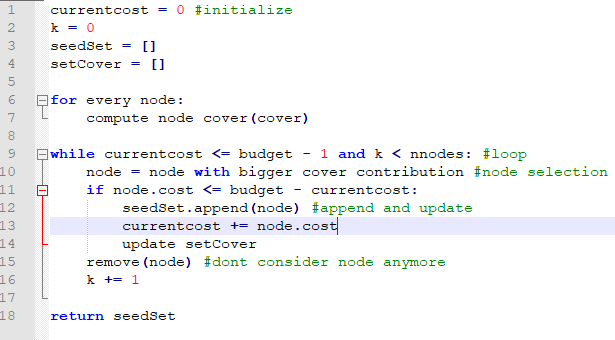
\includegraphics[scale=0.9]{/PseudoCode/maxcoverpseudo}
    \\
    Figure 4.10: Pseudo code For MC function
\end{center}

      \newpage
      \chapter{Results}
\label{cha:conclusion}
Each strategy was tested on three realistic temporal network datasets, with its performance measured and plotted. Different runs were made, with increasing budget value and a fixed Pspread as well as runs with fixed budget and increased Pspread. Each of the runs consisted of a sufficiently high number of simulations (average spread was considered as infection value), to get valid results despite the probability factor. The goal of these tests was to develop a 360° view of the strategies under different point of views, and the following aspects are plotted and showed:
\begin{itemize}
    \item Seed Set Size Characterization with budget increment
    \item Performance variation with budget increment
    \item Performance variation with Pspread increment
    \item Performance variation across the different datasets
    \item Performance comparison between strategies
\end{itemize}
The results are displayed according to the dataset and then discussed together in a final report discussion.

\section{College Message Dataset}
\label{sec:collegeres}
This dataset consisted of a total of 1899 nodes and 59835 edges, each one at a different time (so no simultaneous edges), a decent 31 nodes to edges ratio and roughly 1 percent of unreachable nodes.
\begin{center}
    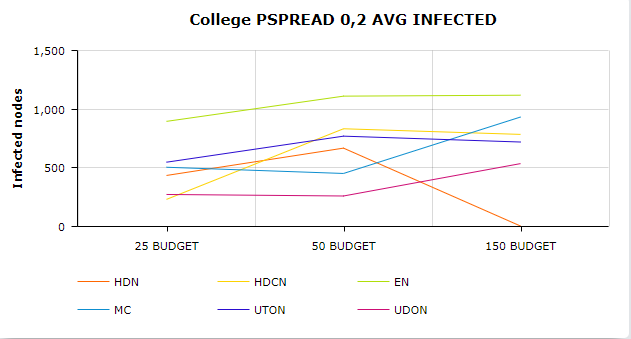
\includegraphics[scale=1]{/resultscollege/college avg performance}
    \\
    Figure 5.1: Overall Performance Of the Strategies on College Dataset
\end{center}

The result shows that the Earliest Nodes strategy was the overall best performing on this dataset(50-60 percent of the nodes). Not only, it was also the only strategy to have a (non-linear) increase of the performance when given more budget, despite the increments not being extremely large.
\begin{center}
    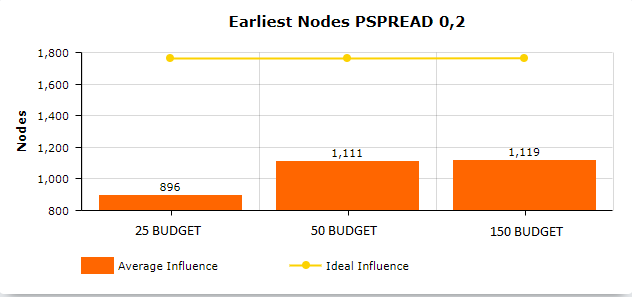
\includegraphics[scale=1]{/resultscollege/earlier performance P02}
    \\
    Figure 5.2: Close Up Performance Of the Earliest Nodes Strategy
\end{center}

This chart shows the progression of the influence with increasing budget, as well as the ideal influence. That is the maximum number of nodes that could have been influenced with this strategy at maximum Probability Pspread = 1. A further run with fixed budget 50 and Pspread = 0.4 was made and it averaged 1417 Infected Nodes (74,6 percent of the nodes). 

\begin{center}
    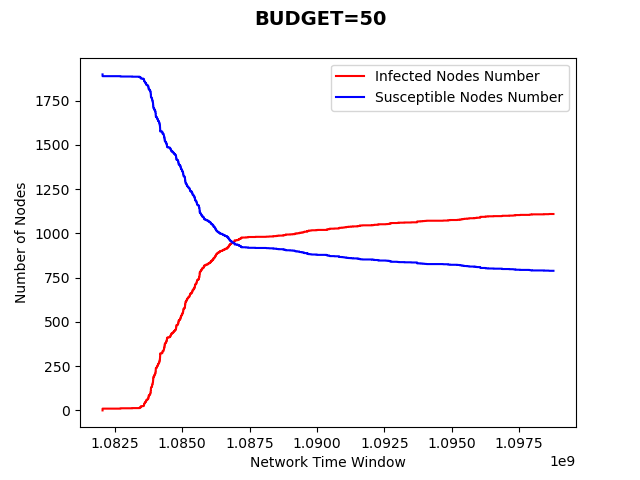
\includegraphics[scale=0.6]{/growth/collegeearlygrowth}
    \\
    Figure 5.3: Curve of Infection for Earliest Nodes PSPREAD 0,2 BUDGET 50
\end{center}
This  chart shows the curve of the infection that the Earliest Nodes Strategy generated with budget 50 and Pspread 0,2. It is easy to see from the chart how the earlier nodes impact the curve; in fact it is growing fast at the beginning and is more linear/stable in the later stages of the simulation. This happens because the seed nodes are highly active in the initial stage of the network, but in the later stages the spreading relies on the actually infected nodes, which are limited to the Pspread value and so the progression is massively slower. What follows is the ideal influence spread growth for the strategy.

\begin{center}
    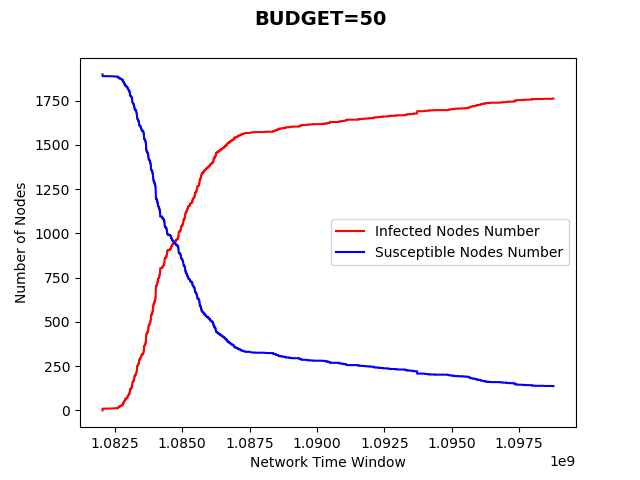
\includegraphics[scale=0.6]{/growth/50-1-college}
    \\
    Figure 5.4: Ideal Curve of Infection for Earliest Nodes PSPREAD 1 BUDGET 50
\end{center}

One noticeable thing is the big downfall of the Highest Degree Nodes Strategy on the test with 150 budget. This is related to one of the main drawbacks of the highest degree strategy: some particular values for the budget can fit exactly one node's cost and therefore the seed set can be small. Moreover, the degree is calculated on the amount of node's messages, meaning that a node with high degree can be also interacting multiple times with the same one node (poor cover). This is something extremely related to the network structure, and as shown in the graph the strategy on 150 budget averaged 4 infected nodes out of 4 maximum infect-able.

\begin{center}
    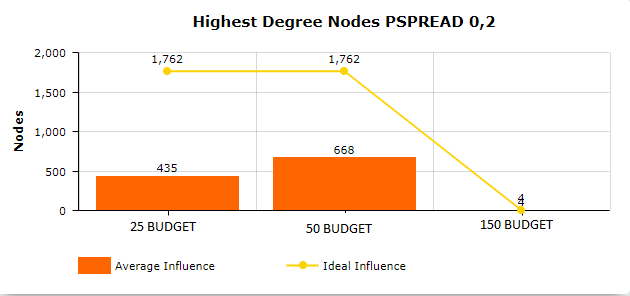
\includegraphics[scale=1]{/resultscollege/greedy performance P02}
    \\
    Figure 5.5: Close Up Performance Of the Highest Degree Nodes Strategy
\end{center}

\begin{center}
    \includegraphics[scale=1]{/resultscollege/seedset}
    \\
    Figure 5.6: Seed Set Size Variation on All Strategies
\end{center}
 The dynamics of the varying node cost also allows seed sets to be not only different in the nodes but also in the overall size. This chart shows that almost every strategy proposed here features an increment of the seed set size with higher budget. This is simply due to the fact that those strategies are not based on picking the highest degree nodes, and more budget allows for more nodes to be seeded, instead of better nodes like in highest degree strategy.

\section{Proximity Conversation Dataset(Ia)}
\label{sec:iares}
This was the strongest connected dataset among all the used ones. It had 20818 edges for only 113 nodes, averaging 184 nodes per edge. Also, only one node in the whole dataset was unreachable or isolated.
\begin{center}
    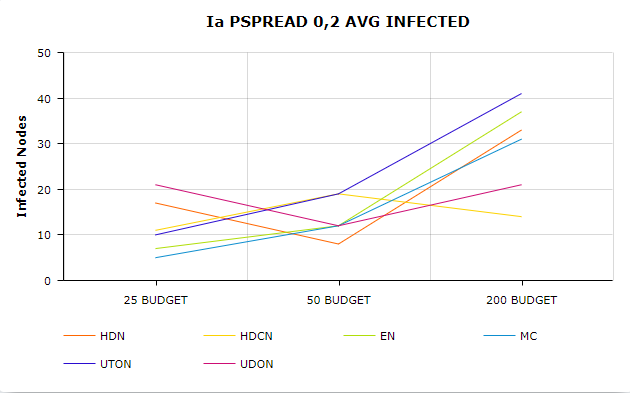
\includegraphics[scale=1]{/resultsia/ia avg performance}
    \\
    Figure 5.7: Overall Performance Of the Strategies on Proximity Dataset Ia
\end{center}

What emerges from the chart is that whatever the budget was, the best strategy was always one of the two that focus on the hardest nodes to reach. That makes sense, because on a strongly connected network like this the majority of the nodes is going to have high in degree, making them getting infected most likely even if they are not seeded or neighbors of the seed nodes. Those strategies allow to include also nodes that are most likely going to be cut out of the network, resulting in an overall better performance as predicted when introducing this network type. \\
However, there were a lot of nodes that were harder to reach than others, and this is shown by the fact that the two strategies based on those nodes had drastically different results at each run. Also, the evolution shows that as the budget increased, the strategies that evolved node degrees were the worst performing, while on lower budget it was the exact opposite.

\begin{center}
    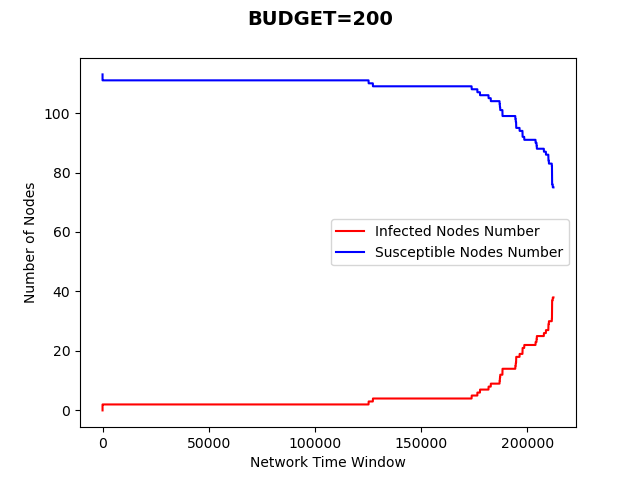
\includegraphics[scale=0.6]{/growth/ia}
    \\
    Figure 5.8: Curve of Infection for Unreachable, Time Oriented Nodes Strategy PSPREAD 0,2 BUDGET 200
\end{center}
The curve clearly reveals some details regarding the structure of the network: the most difficult nodes to reach (the ones with less edges going into them) are all activated in the later to final stages of the network, showing that no relevant Infected - Susceptible interactions occurred during the entire first half of the temporal window, resulting in a potential "waste". However the strategy was still the best on medium-higher budget scenarios.

\begin{center}
    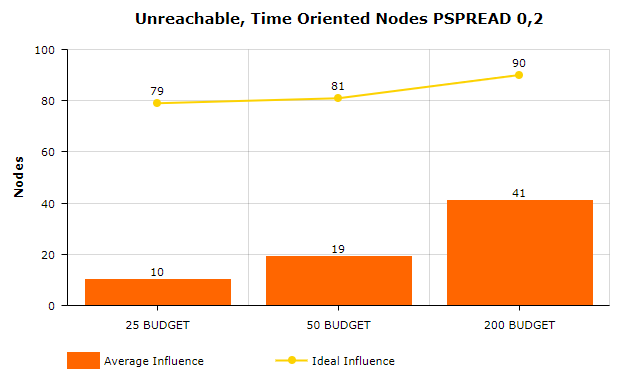
\includegraphics[scale=0.8]{/resultsia/uton performance P02}
    \\
    Figure 5.8: Close Up Performance Of the Unreachable, Time Oriented Nodes Strategy
\end{center}

On this particular dataset the majority of the strategies had a consistent increment of performance with more budget, especially when going from low budgets to a decent budget like 200.

\begin{center}
    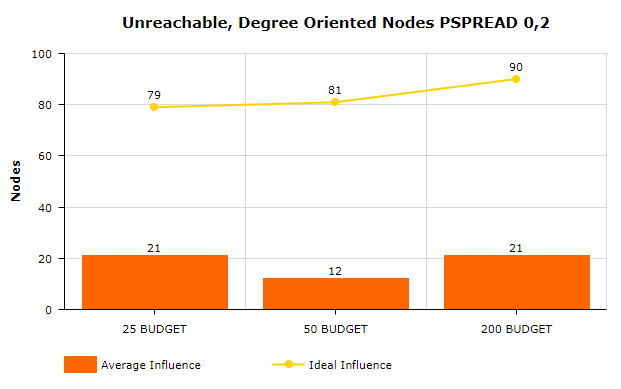
\includegraphics[scale=0.8]{/resultsia/udon preformance P02}
    \\
    Figure 5.9: Close Up Performance Of the Unreachable, Degree Oriented Nodes Strategy
\end{center}

It is interesting to see the big difference between the two Unreachable Nodes oriented strategies. What emerges from the charts is that generally, when the budget is lower the degree of the nodes seems to have more impact in determining the overall performance, whilst with higher budgets the temporal aspect of the networks really make a great difference. On medium-high budget scenarios the worst performing strategy is always some degree related one.

\begin{center}
    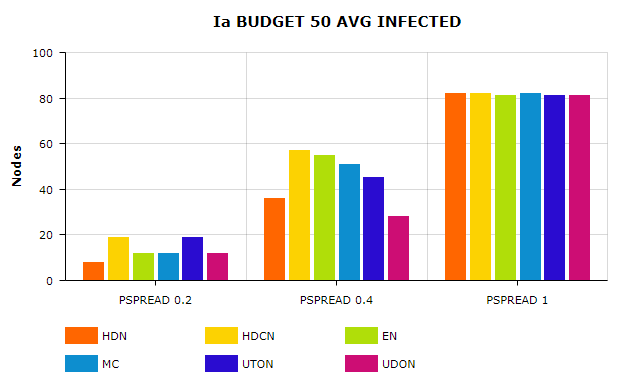
\includegraphics[scale=1]{/resultsia/ia performance prob}
    \\
    Figure 5.10: Performance Variation with increasing Probability
\end{center}

This chart shows that on a highly connected dataset like this one, the overall max performance of each strategy is very similar, however when scaling with the probability spread without saturation there are strategies that get really drastic improvement. These strategies are the ones that either do not consider the quality of the nodes like Maximum Cover Nodes Strategy or the ones that can involve very high-risk high-reward nodes, like the degree based strategies. What generally emerged is that Probability is by far more impactful in a strategy's performance compared to the budget cap.

\section{Chat Dataset(SFHH)}
\label{sec:sfhhres}
This dataset was strongly connected as well, averaging 174 edges per node on a total of 403 nodes. The total number of edges was over 70k, and these were pretty homogeneously distributed between the nodes, as the maximum reach of ideal infection was nearly the same for all the strategies on each run. This made the seed choice even more impactful for the spreading performance. Finally, this network had only 5 unreachable nodes.
\begin{center}
    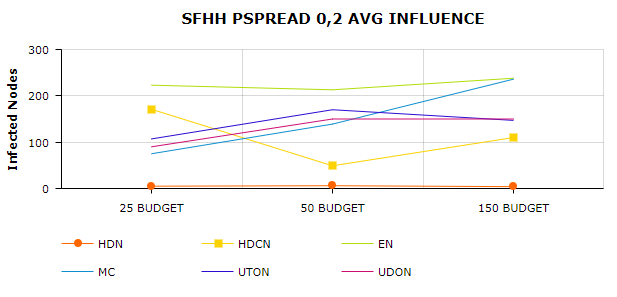
\includegraphics[scale=1]{/resultssfhh/avgperformance}
    \\
    Figure 5.11: Overall Performance Of the Strategies on Chat Dataset SFHH
\end{center}

As the chart shows, the Earlier Nodes strategy was consistently the best, with only the Maximum Cover strategy coming close to it on the higher budget run, but still not topping it. Degree based strategies proved to be generally the worst, with generic highest degree strategy showing an awful performance, while both Unreachable Node based Strategies were solid third and fourth place in every run. It is also noticeable how their values are closer than in every other dataset, and that is because with this particular network structure the unreachable nodes were exclusive, which means there were no nodes with equal low in-degree which is what leads to the strategies always seeding the same nodes. The slight gap in the performance is given by the fact that the average Infection is calculated on a finite number of runs, and it can be a little bit off but not enough to compromise the results. 


\begin{center}
    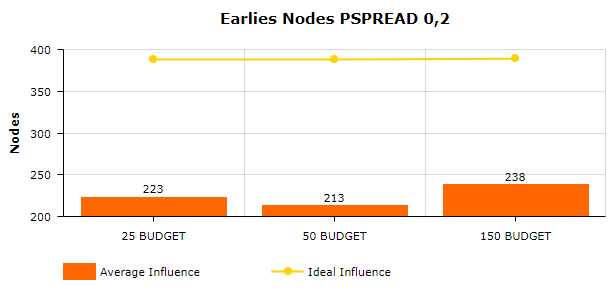
\includegraphics[scale=1]{/resultssfhh/early performance}
    \\
    Figure 5.12: Close Up Performance Of the Earlier Nodes Strategy
\end{center}

An interesting thing here is that despite being the best among the strategies on each single run, averaging 56 percent of total nodes infected, this strategy did not show any important performance boost when fed with more budget. We have learned from previous data sets that budget cap can be tricky, because it can allow higher degree nodes to be seeded that might can have less impact than expected on the influence spread.
\\
Also, being a strongly connected network made every strategy have similar ideal influence results (roughly 95-96 percent of the total nodes, however only EN averaged more than 50 percent of actually influenced nodes on each run, meaning that a correct seed set choice was very crucial. 
\\
\\
Another interesting observation is the curve of infection generated by this strategy, which merges the spreading of the best strategies on the other datasets: in fact, here the curve presents a fast growth in the initial stages of the network, as the strategy is supposed to, followed by a stalling phase in the entire mid range of the network and a final growth again in the later stages.

\begin{center}
    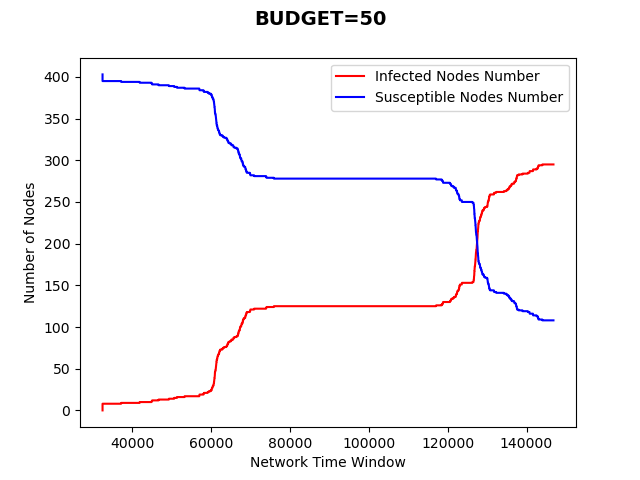
\includegraphics[scale=0.8]{/growth/testgrowth}
    \\
    Figure 5.13: Curve Of Infection for the Earlier Nodes Strategy
\end{center}

The seed set size behaviour was also really interesting: in this dataset the seed sets were generically small on the highest budget run, as going from 50 to 150 budget characterized a drop in the seed set cardinality from values around 8 to seed sets of 1 or 2 nodes, except for two strategies who had pretty consistent seed set size. This enabled nodes of cost just slightly under the budget cap to be seeded, dropping the cardinality by a lot; noticeable is how this did not happen in EN and MC, giving us further information on the network structure. Earlier nodes were generally cheaper, and the cascades generated by them were the ones maximizing the nodes cover, although the seed sets of the two strategies was different by just one node.
This allows us to claim that this network was strongly time dependent, meaning that the earlier nodes were the best both for covering the network but also for actually maximizing the spread of influence.

\begin{center}
    \includegraphics[scale=0.8]{/resultssfhh/seedset}
    \\
    Figure 5.14: Seed Set Size Variation with increasing Budget
\end{center}
      \newpage
      \chapter{Conclusions}
\label{cha:conclusion}
In this last chapter a general overview of the project is given with regard to the results collected, the observations made and the direction where future works and developments of this project will be oriented, with some of them already being introduced in the past chapters. 
\\
The main goal of the project was to provide a suitable Influence Maximization model for realistic temporal networks, under particularly restricting budget and computational constraints. The most important thing was to analyze the model and see if good results were achievable under those mentioned limitations, and underline correlations between network structures and specific solution approaches.
\\ 
As said earlier, temporal networks lead to new challenges for algorithm design and bring a new dimension to the problems. As predicted, these changes have an enormous impact on problems like Influence Maximization, with the results clearly underlining that applying classic solutions for static networks on temporal networks is not the way to go as in zero tests a degree only based strategy had the best average influence nor ideal influence.\\
However, it has been clearly proved that the temporal aspect in networks does not only impact nodes' ordering, but also the nodes' reachability and cascade cover. The goal was to underline any correlation between networks features and an optimal solution based on those features. \\
Overall, choosing the nodes by time of activation was the best among the proposed solutions. One particular observation about this strategy is that in some runs it did not show much of an improvement even with higher budget, possibly underlining the fact that, in most network models, earlier nodes have more time to activate therefore have higher degree and only a few of them are selectable, which brings the extra budget to be used in mid/late nodes with lower degree. \\
Also, one of the goals of this work was to study an eventual correlation between budget and performance, and between budget and seed set size. Overall, increasing budget brought general performance boost. However the progress was not linear at all, with strategies clipping from 50 to 150 budget, and most remarkable performance boosts coming with 200 budget. The designed strategies have been budget-optimized not to waste budget on nodes in any of the seed nodes' neighbors, however it is clear that deeper node quality classification needs to be implemented in future works, as for example when seeding a node with 5 degree there were no considerations made on how many nodes that degree was distributed on from 1 to 5.\\
This is also related to the impact of the seed set size on the average infection, as seed sets with equal cardinality can have a much bigger neighbors set than others.
As expected, strategies born on purpose for highly connected network models like UDON and UTON averaged solid results on those type of networks revealing that focusing on that aspect of the network was a good call. \\
Overall, there was no linear relation between budget cap and seed set size, as the strategies were all greedy based, which makes the seed sed size be related to how close to the budget cap the best node for each strategy is. A budget of 150 was set so that 5 degree nodes would come close to it, allowing for a very restricted set on degree based strategies. However not only those strategy presented runs with lower seed set cardinality.
\\ 
Correlation between Probability of spread and performance was also analyzed, already knowing that it would bring a consistent boost in general infection spread. It turned out to be much more impactful than budget boost, and as predicted the strategy of Maximum Cover was the one with the best scaling of performance along the Probabilty. However at saturation Probability = 1 the strategies were very similar if not identical in cover on highly connected networks, with some slightly more important difference in the College Dataset, which was the one with the least nodes to edges ratio. 
An interesting observation on the result is the absence of correlation between a dataset's nodes to edges ratio and the average performance of the better working strategy on that dataset, as the runs on the Ia dataset show.

$\\$

To conclude, the work brought positive results, as it shows that for each dataset it is possible to develop some low computational cost functions that can produce a solid 50ish and even more percent of influenced nodes across the network. The extremely limited budget and fast growing node cost make those results really good to be applied in real life large scale social networks.\\
Finally it has been showed that further implementations need to be made for the strategies to enhance even more their performance and adapt them to every temporal network type, as some of them do not include some aspects or do not differentiate the node choice enough. On top of that, new strategies designed as good compromises between two or more of these proposed ones can be implemented to suit generic network models or to serve their purpose on even more limited tests, like limited network knowledge.
\\
Future works will aim at enhancing even more the realistic aspect of both the seeding, like reduced network knowledge, and the simulation aspect, implementing trust dynamics between nodes and variable spreading on influence between two nodes interacting. Also, more in-depth solutions will be studied, always withing a certain limit of computation cost. An interesting work is to bring this study to higher order networks or hypergraphs
\cite{https://doi.org/10.48550/arxiv.2206.01394}, whose study is extremely important because they are the best mathematical structure that can fit a social interaction model thanks to the multiple nodes per edge property, allowing to insert group dynamics into social network influence models.
      \newpage
    
      
      
    \endgroup


    % bibliography - bibtex format
    %
    % add chapter to index
    \addcontentsline{toc}{chapter}{Bibliography}
    % alphabetical order of authors
    \bibliographystyle{plain}
    \bibliography{biblio}
%%%%%%%%%%%%%%%%%%%%%%%%%%%%%%%%%%%%%%%%%%%%%%%%%%%%%%%%%%%%%%%%%%%%%%%%%%
%%%%%%%%%%%%%%%%%%%%%%%%%%%%%%%%%%%%%%%%%%%%%%%%%%%%%%%%%%%%%%%%%%%%%%%%%%
%% Nota
%%%%%%%%%%%%%%%%%%%%%%%%%%%%%%%%%%%%%%%%%%%%%%%%%%%%%%%%%%%%%%%%%%%%%%%%%%
%% In the bibliography, all the sources consulted for the dissertation 
%% have to be cited and listed in alphabetical order by the 
%% first author's surname.
%%
%% According to the source material, the quotation has to be as follows:
%%
%% BOOKS
%% Surname and initial/s of the name/s of the author/s, date of edition,
%% publishing house and (if applicable) number of edition.
%% 
%% JOURNAL ARTICLES 
%% Surname and initial/s of the first name/s of the author/s,
%% title of the article, name of the journal, volume number, issue number
%% and page numbers.
%% 
%% CONFERENCE PAPERS
%% Surname and initial/s of the name/s of the author/s,
%% year of the conference, title of the article, name of the conference,
%% place of the conference, conference dates, page numbers.
%% 
%% CITING WEB RESOURCES
%% The consulted webpages have to be listed in alphabetical order. 
%% It is necessary to:
%%   - Copy the specific URL (the web address) of the consulted webpage
%%   - If available, indicate the surname and first name of the author/s,
%%     the title and subtitle of the text
%%   - If available, indicate the last date you retrieved the webpage
%%     (day/month/year).   
%%%%%%%%%%%%%%%%%%%%%%%%%%%%%%%%%%%%%%%%%%%%%%%%%%%%%%%%%%%%%%%%%%%%%%%%%%
%%%%%%%%%%%%%%%%%%%%%%%%%%%%%%%%%%%%%%%%%%%%%%%%%%%%%%%%%%%%%%%%%%%%%%%%%%
    

    

\end{document}
